\documentclass{article}
\usepackage{times, graphicx}
\usepackage[utf8]{inputenc}

\begin{document}

\title{Project Proposal \\
      Brai(a)n \\
      - \\
      An AI who learn}
\author{Alexandre Fulgoni \\
        Stéphane Nguyen \\
        Sebastien Maire \\
        Thomas Nieto \\
        - \\
        Epitech 2017 \\
        Paris \\
}


\date{\today}
\maketitle
\begin{center}
  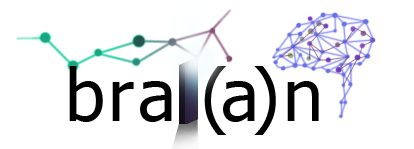
\includegraphics[scale=0.5]{braian}
\end{center}

\clearpage

\section{Introduction}
  Le but de ce pfa\footnote{coucou} est de réaliser une intelligence artificielle. \\
  IA étant vaste, nous nous concentrons sur l’apprentissage \\
  Notre projet se concentrera sur l’aspect apprentissage et prise de décision.
  Environnement Minecraft - Terraria - Spelunky

\section{Equipe}
  \begin{description}
    \item[Sébastien Maire] \hfill \\
      \textbf{Chef Technique} \\
      Application de connaîssances
      en algorithmie et leur approndissement
    \item[Alexandre Fulgoni] \hfill \\
      \textbf{technique} \\
      l’IA a toujours été un domaine vers lequel Alexandre a
      toujours voulu travailler, ce pfa s’est tout naturellement posé
      comme
    \item[Stéphane Nguyen] \hfill \\
      \textbf{technique} \\
      intéressé par le développement de jeu-vidéo. En effet,
      au-delà du graphisme, l’IA est LE pillier qui permet le réalisme
      et donc l’immersion du joueur.
    \item[Thomas Nieto] \hfill \\
      \textbf{Recherche et managment} \\
      ...
  \end{description}

  Première fois ensemble dans un groupe. Nous nous sommes rencontrés grâce aux
  intérêts que nous partageons et sommes donc tous motivés pour aller le plus
  loin possible.

\section{Contexte}
  Ce projet n’a pas pour vocation d’être distribué à des fins commerciales.
  C’est purement un
  projet de R\&D en partenariat avec le HUB.
  Utilisation d’algorithmmes d’apprentissage et application dans un monde
  virtuelle pour la démo pour nous : Apprentissage / découverte et
  application de l’IA

\section{Partenaire}
  HUB

\section{Objectifs}
  Coupler prise de décision et apprentissage
  Cas concret : arbre de décision qui change ses nodes.


\section{Planning}
  2 jours par semaine : Samedi et dimanchehey


\end{document}
% # Introduction
%% Le but de ce pfa est de réaliser une intelligence artificielle.
%
% <AI étant vaste, nous nous concentrons sur l’apprentissage>
% Notre projet se concentrera sur l’aspect apprentissage et prise de décision.
%
%
% Environnement Minecraft - Terraria - Spelunky

%
% # Equipe
% * Sebastien Maire
%     * chef technique
%     * appliquer des connaissances en algorithmie et les approfondir
%     grace à un cas concret qu’est ce pfa
% * Alexandre Fulgoni
%     * technique
%     * l’IA a toujours été un domaine vers lequel a toujours voulu travailler dans l’IA, ce pfa s’est tout naturellement posé
% * Stephane Nguyen
%     * technique
%     * intéressé par le développement de jeu-vidéo. En effet, au-delà du graphisme, l’IA est LE pillier qui permet le réalisme et donc l’immersion du joueur.
% * Thomas Nieto
%     * recherche et manager d’equipe
%     * ...
%
% Première fois ensemble dans un groupe. Nous nous sommes rencontrés grâce aux intérêts que nous partageons et sommes donc tous motivés pour aller le plus loin possible.
%
%
% # Contexte
% Ce projet n’a pas pour vocation d’être distribué à des fins commerciales. C’est purement un
% projet de R&D en partenariat avec le HUB.
% Utilisation d’algorithmmes d’apprentissage et application dans un monde virtuelle pour la démo
% pour nous : Apprentissage / découverte et application de l’IA
%
% # Partenaire
% HUB
%
% # Objectifs
% Coupler prise de décision et apprentissage
% Cas concret : arbre de décision qui change ses nodes.
%
% # Planning général
% 2 jours par semaine : Samedi et dimanche
